\documentclass[pdf]{beamer}
\usepackage{caption}

\newcommand{\Wx}{\Omega_x}
\newcommand{\Wy}{\Omega_y}
\newcommand{\CW}{^{\mathrm{CW}}}
\newcommand{\CCW}{^{\mathrm{CCW}}}
\newcommand{\MDM}{^{\mathrm{MDM}}}
\title{Modeling of CW/CCW calibration in a FS-type lattice}
\author{Alexander Aksentev}

\begin{document}
	\begin{frame}
		\titlepage
	\end{frame}
	\begin{frame}
		\frametitle{Overview}
		\begin{itemize}
			\item Optimization of sextupole strengths for reducing decoherence;
			\begin{itemize}
				\item problem with simultaneous suppression of x- and d-offset decoherence.
			\end{itemize}
			\item Modeling of the CW/CCW calibration procedure;
			\begin{itemize}
				\item spin freeze problem.
			\end{itemize}
		\end{itemize}
	\end{frame}
	\begin{frame}
		\frametitle{Optimization of sextupole strengths}
		\framesubtitle{for the reduction of decoherence}
		\begin{itemize}
			\item Three sextupole families (GSX, GSY, GSD), each expected to suppress decoherence, resp., in X-,Y-,D-planes;
			\item spin tune Taylor expansion (COSY Infinity) assumes the form (some terms omitted): 
			\[
				\mu(x,y,d) = \mu_0 + a_{xx}\cdot x^2 + a_{yy}\cdot y^2 + a_{dd}\cdot d^2 + a_{xd}\cdot x\cdot d + a_{yd}\cdot y\cdot d;
			\]
			\item parabolic dependence of spin tune on the $x,y,d$ variables (confirmed by spin tracking) $\Rightarrow$ objective function $f = a_{xx}^2 + a_{yy}^2 + a_{yd}^2$;
			\item the reason $a_{dd},~ a_{xd}$ are not involved in $f$: $a_{xx},~a_{dd}$ couldn't be minimized simultaneously (analysis below).
		\end{itemize}
	\end{frame}
\begin{frame}\frametitle{Computed as $\mu_i = \mu(x_0^i,y_0^i,d_0^i)$}
	\centering
	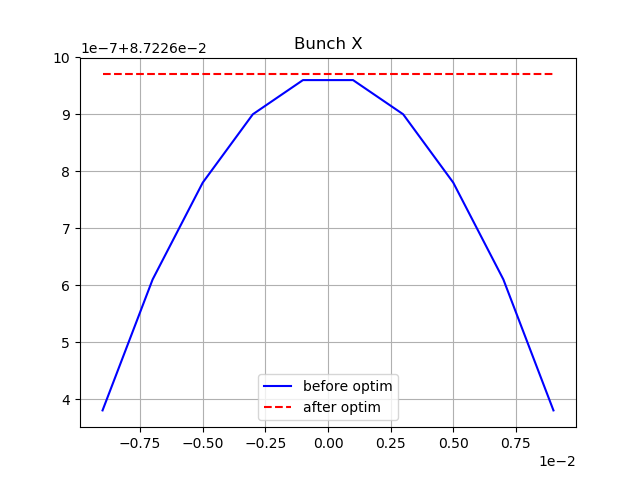
\includegraphics[scale=.33]{decoh/Xbunch/Wy_vs_Xdecoh0_}%
	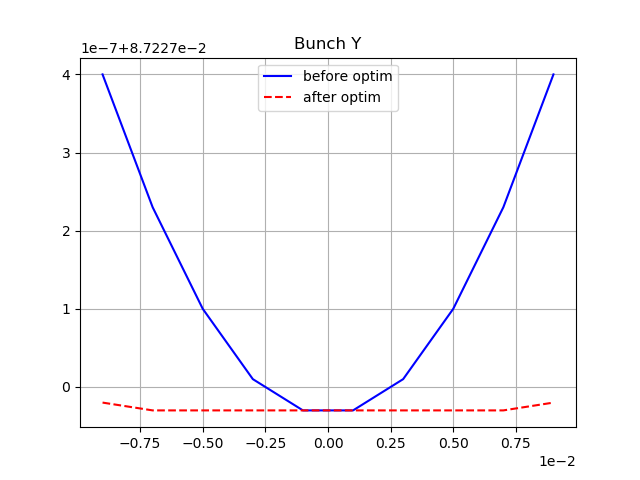
\includegraphics[scale=.33]{decoh/Ybunch/Wy_vs_Ydecoh0_}
	
	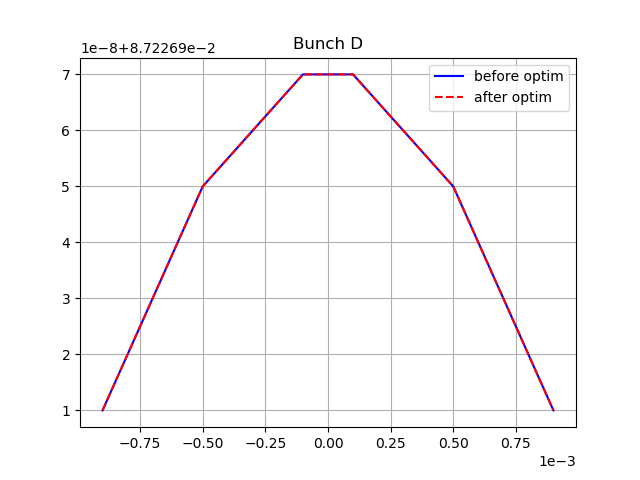
\includegraphics[scale=.33]{decoh/Dbunch/Wy_vs_Ddecoh0_}
\end{frame}
\begin{frame}\frametitle{Linear fit of tracking data}
\centering
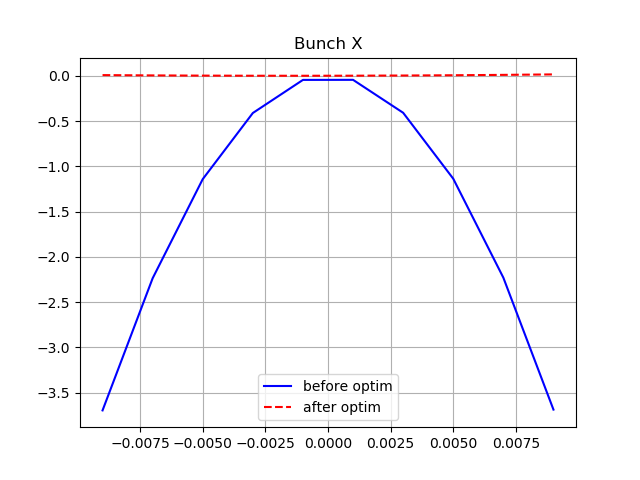
\includegraphics[scale=.33]{decoh/Xbunch/Wy_vs_X_decoh}%
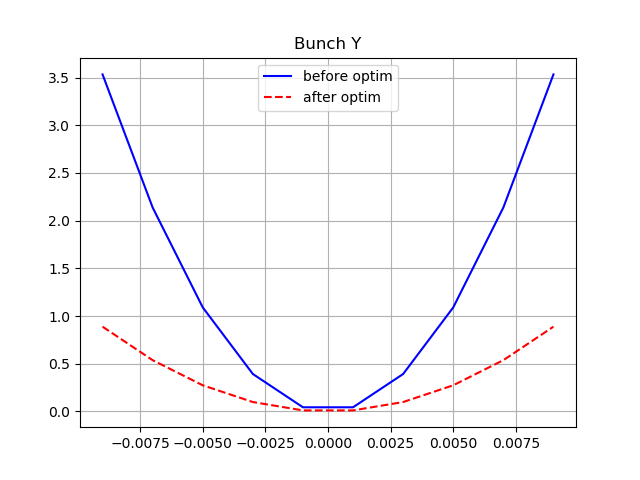
\includegraphics[scale=.33]{decoh/Ybunch/Wy_vs_Y_decoh}

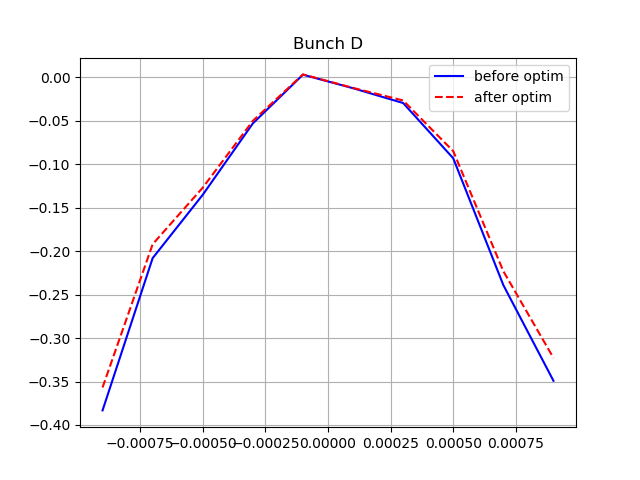
\includegraphics[scale=.33]{decoh/Dbunch/Wy_vs_D_decoh}
\end{frame}
\begin{frame}
	\frametitle{Example fits (X-,D-bunch)}
	\centering
	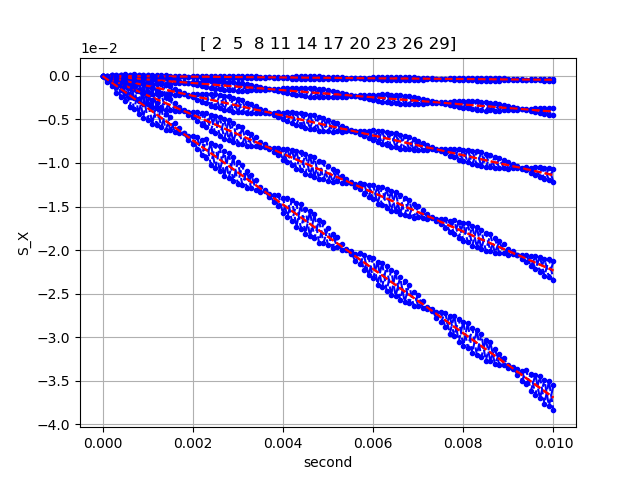
\includegraphics[scale=.33]{decoh/Xbunch/Sx(unoptim)_for_X_bunch_decoh}
	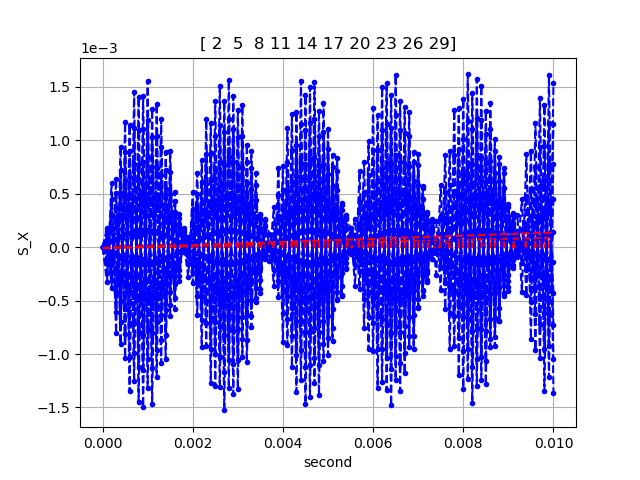
\includegraphics[scale=.33]{decoh/Xbunch/Sx(optim)_for_X_bunch_decoh}
	
	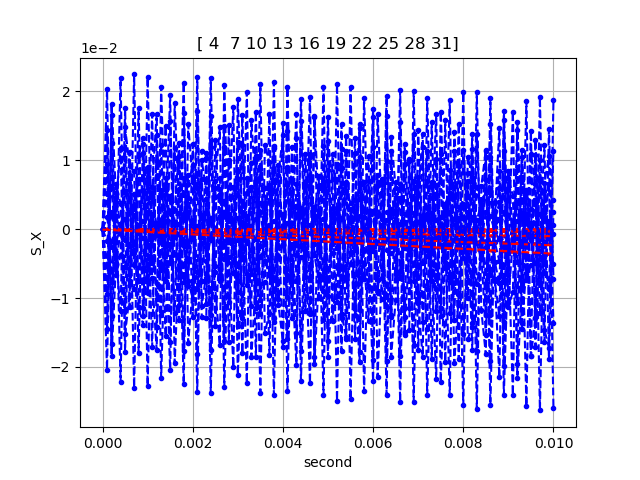
\includegraphics[scale=.33]{decoh/Dbunch/Sx(unoptim)_for_D_bunch_decoh}
	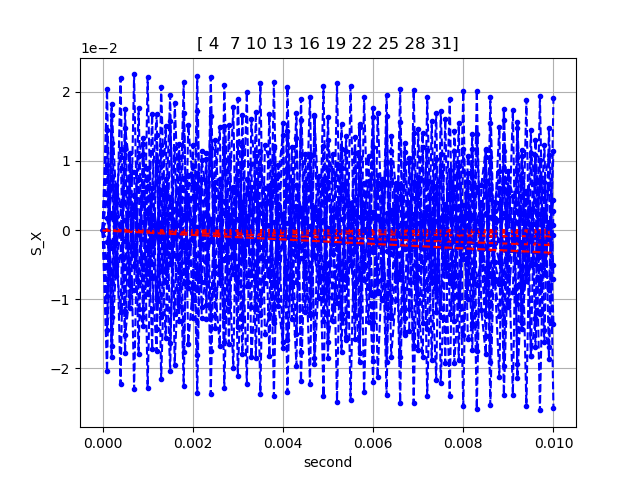
\includegraphics[scale=.33]{decoh/Dbunch/Sx(optim)_for_D_bunch_decoh}
\end{frame}
	\begin{frame}
		\frametitle{Gradient sweep analysis}
		\framesubtitle{FS-type lattice beta functions}
		\begin{itemize}
			\item Sextupoles are placed in the maximums of the corresponding beta functions;
			\item because DispX, BetaX maxima coincide, considered 3 cases: 1) GSD only in big DispX maxima, 2) GSD only in smaller maxima not coinciding with BetaX maxima, 3) GSD in both types DispX maxima.
		\end{itemize}
		\centering
		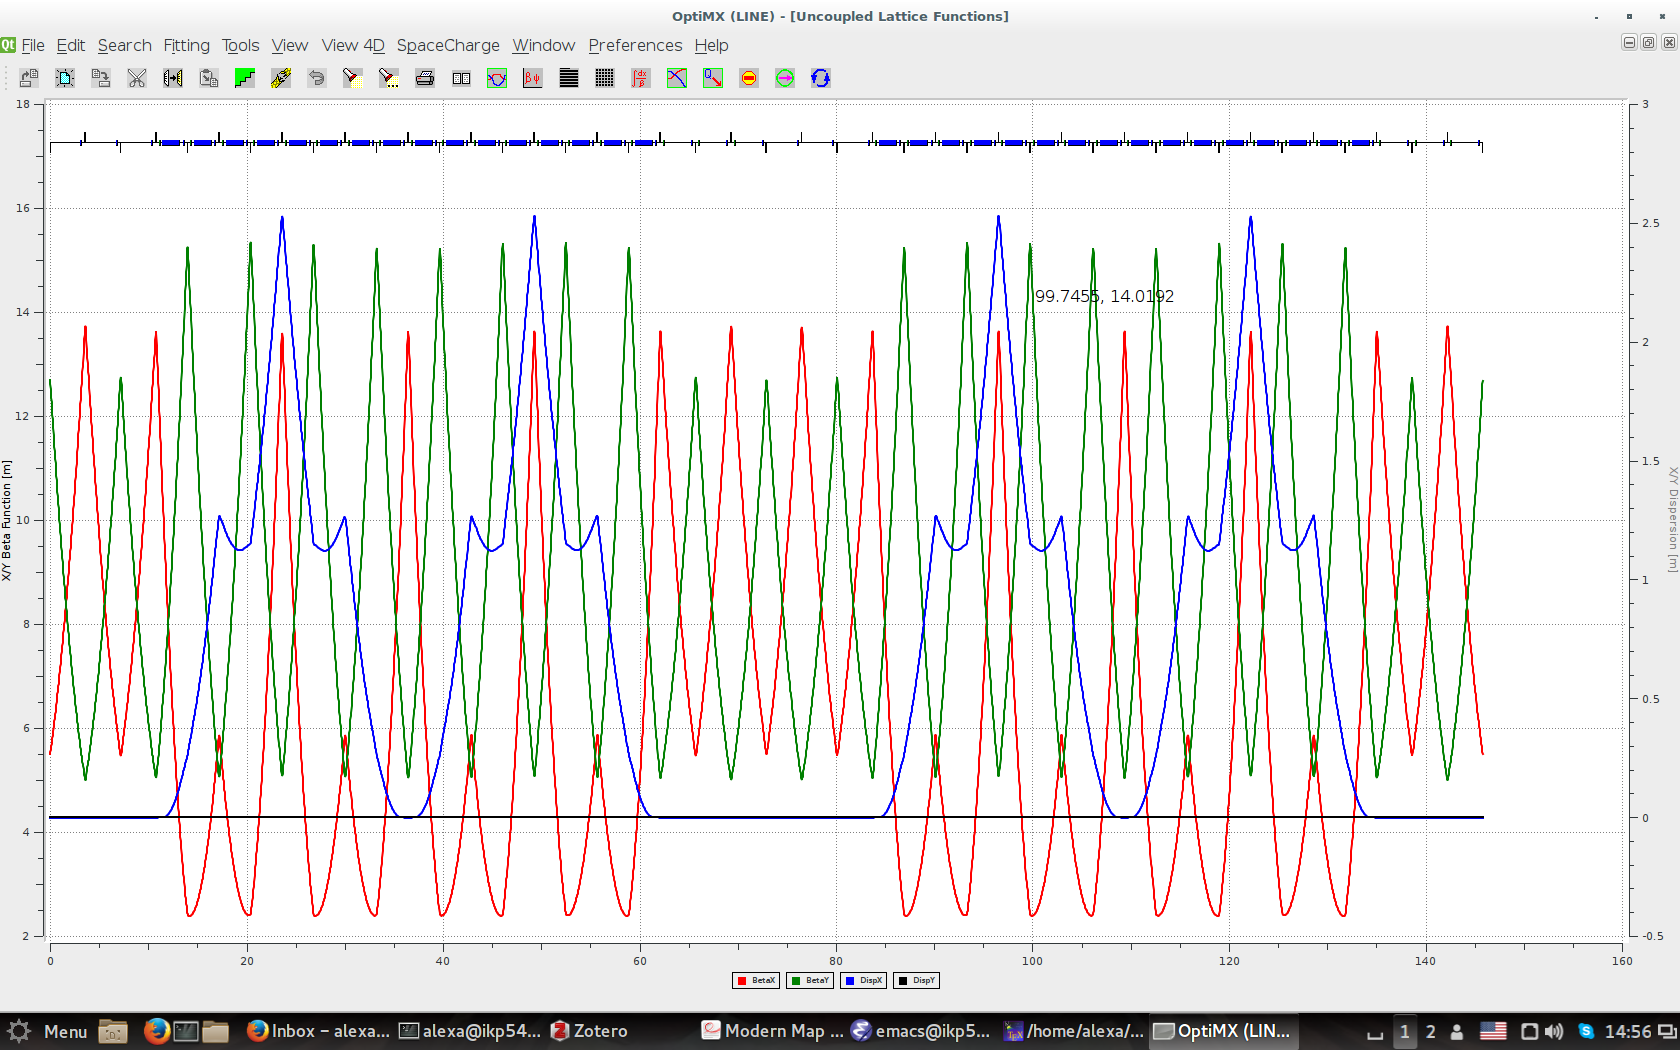
\includegraphics[scale=.12]{FS_BNL_optim}
	\end{frame}
	\begin{frame}\frametitle{Gradsweep cases 4\&12}
	\begin{minipage}{.3\textwidth}
		\begin{itemize}
			\item Took a grid GSX, GSY, GSD: $\pm 10^{-2}$ T/cm$^2$ (10 points each axis);
			\item computed the spin tune, and extracted the $a_{xx}$, $a_{yy}$, $a_{dd}$ coefs (plotted);
			\item observe that $a_{xx}$, and $a_{dd}$ cannot be simultaneously set to 0.
		\end{itemize}
	\end{minipage}
	\begin{minipage}{.65\textwidth}
		\centering
		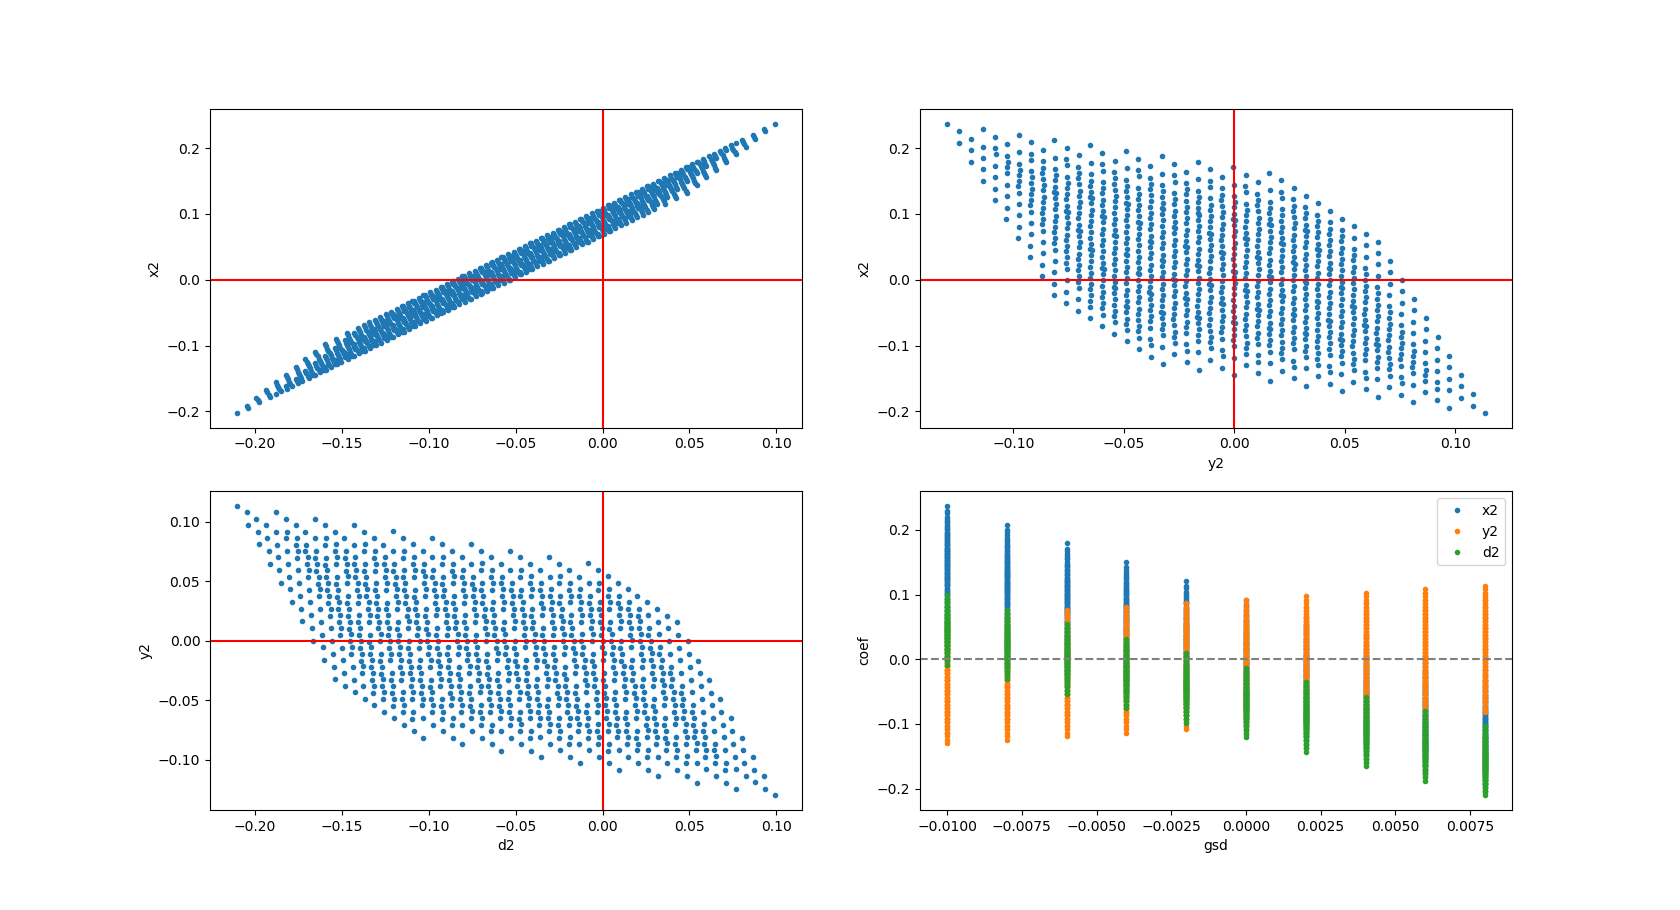
\includegraphics[scale=.19]{decoh/gradsweep_4gsd}
		
		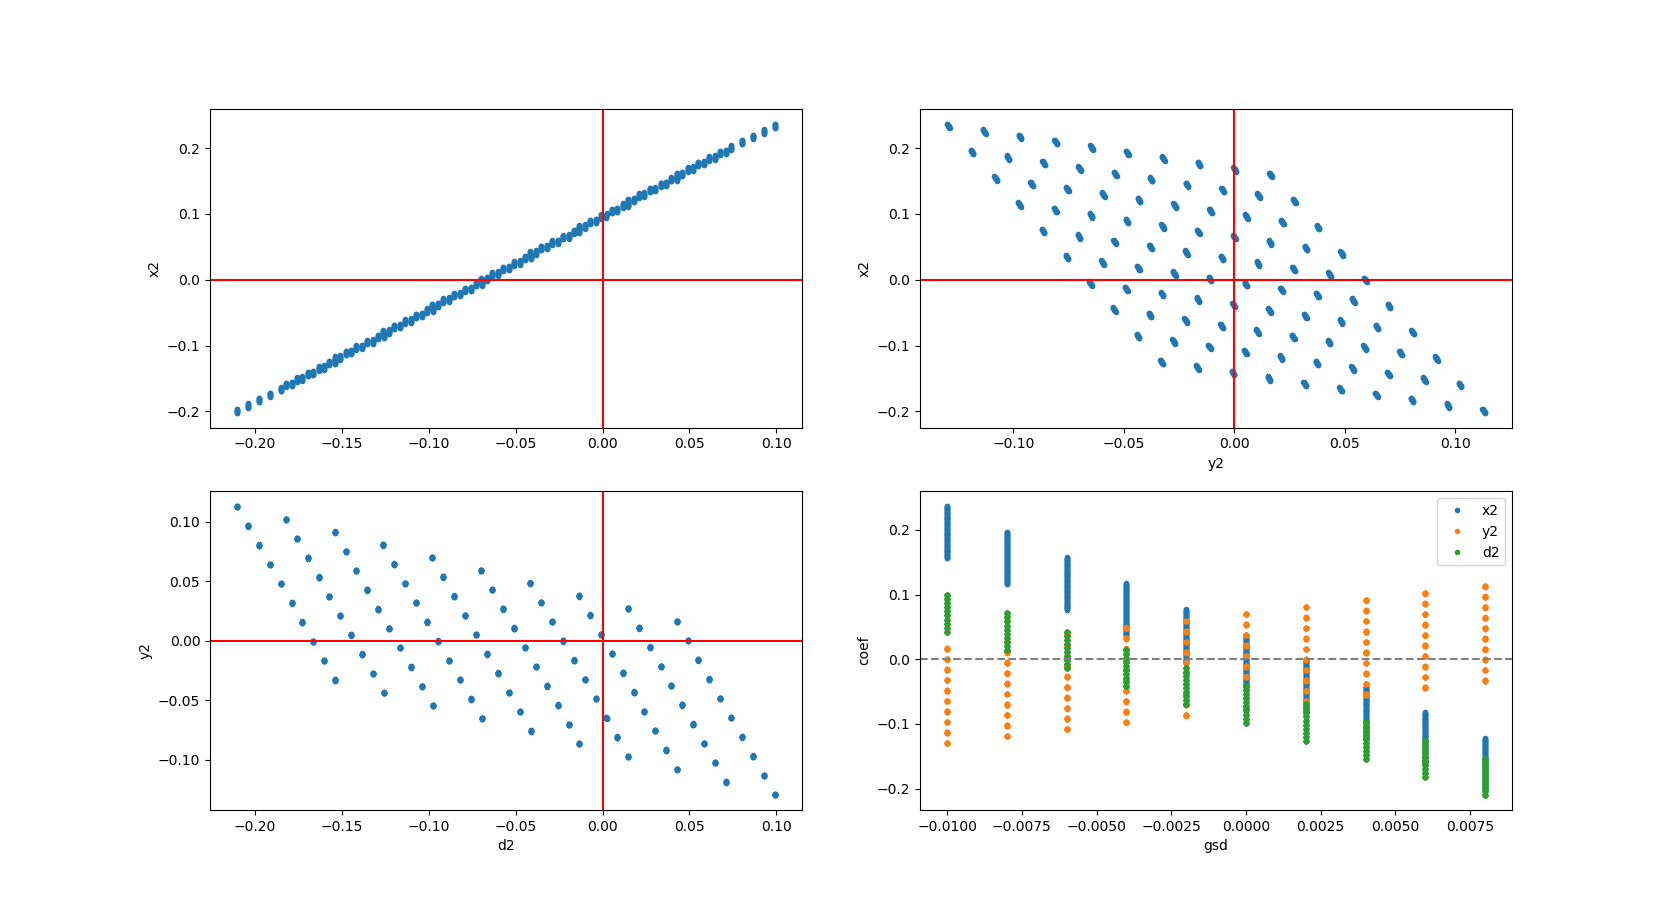
\includegraphics[scale=.19]{decoh/gradsweep_12gsd}
	\end{minipage}
	\end{frame}
	\begin{frame}
		\frametitle{CW/CCW B-field calibration procedure}
		\framesubtitle{Rationale}
		\begin{itemize}
			\item The core idea of the procedure is to use the x-z plane spin precession frequency as a measure of the B-field;
			\item an element tilt $\theta$ introduces a $B_x$ field component, which induces a $\Wx\MDM \propto B_x$;
			\item $\Wy\MDM \propto B_y$, and $B_y ~\text{and}~ B_x$ are strictly related via $\theta$;
			\item $\theta$ doesn't change going from CW to CCW, hence by reproducing $\Wy\MDM$ we can be sure to reproduce $B_y$, and also $B_x$ and $\Wx\MDM$.
		\end{itemize}
	\end{frame}
\begin{frame}
	\frametitle{CW/CCW B-field calibration procedure}
	\framesubtitle{Modeling}
	\begin{enumerate}
		\item distribute element tilt errors $\theta \sim N(\mu_j, \sigma_j), j \in J$;
		\item for an ensemble of initial conditions $\lbrace (x^i,a^i,y^i,b^i,t^i,d^i)\rbrace_{i\in I}$ compute array of $\lbrace(\Wx^i, \Wy^i)\rbrace_{i\in I}$;
		\item compute statistics: $S_1 \equiv |\Wx\CW| - |\Wx\CCW|,~ S_2 \equiv |\Wy\CW| - |\Wy\CCW|$;
		\item repeat for $j \in J$.
	\end{enumerate}
\end{frame}
\begin{frame}\frametitle{Spin freeze}
	\framesubtitle{$\theta = \theta_0$}
	All WF are tilted by the same angle $\theta_0$; $S_y$ oscillates as expected.
	\centering
	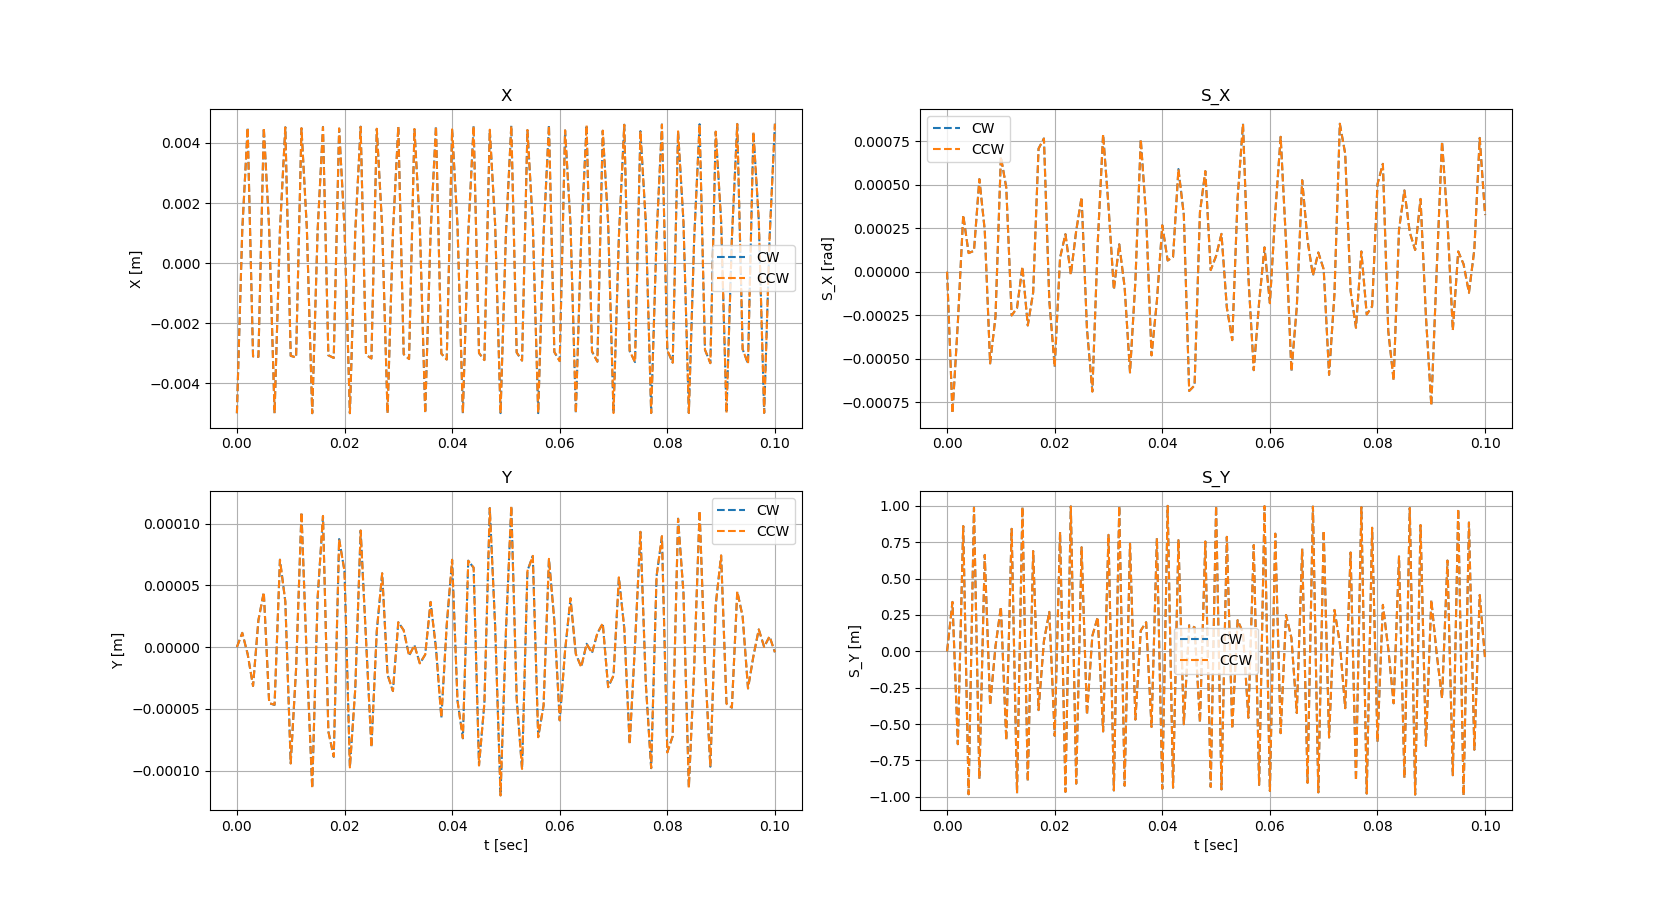
\includegraphics[scale=.3]{freeze/CALIB_ALL_WF_SAME_ANGLE}
\end{frame}
\begin{frame}\frametitle{Spin freeze}
	\framesubtitle{$\theta \sim N(0, \sigma)$}
	Reaching the apex, spin freezes at $(S_y, S_z) = (1, 0)$.
	\centering
	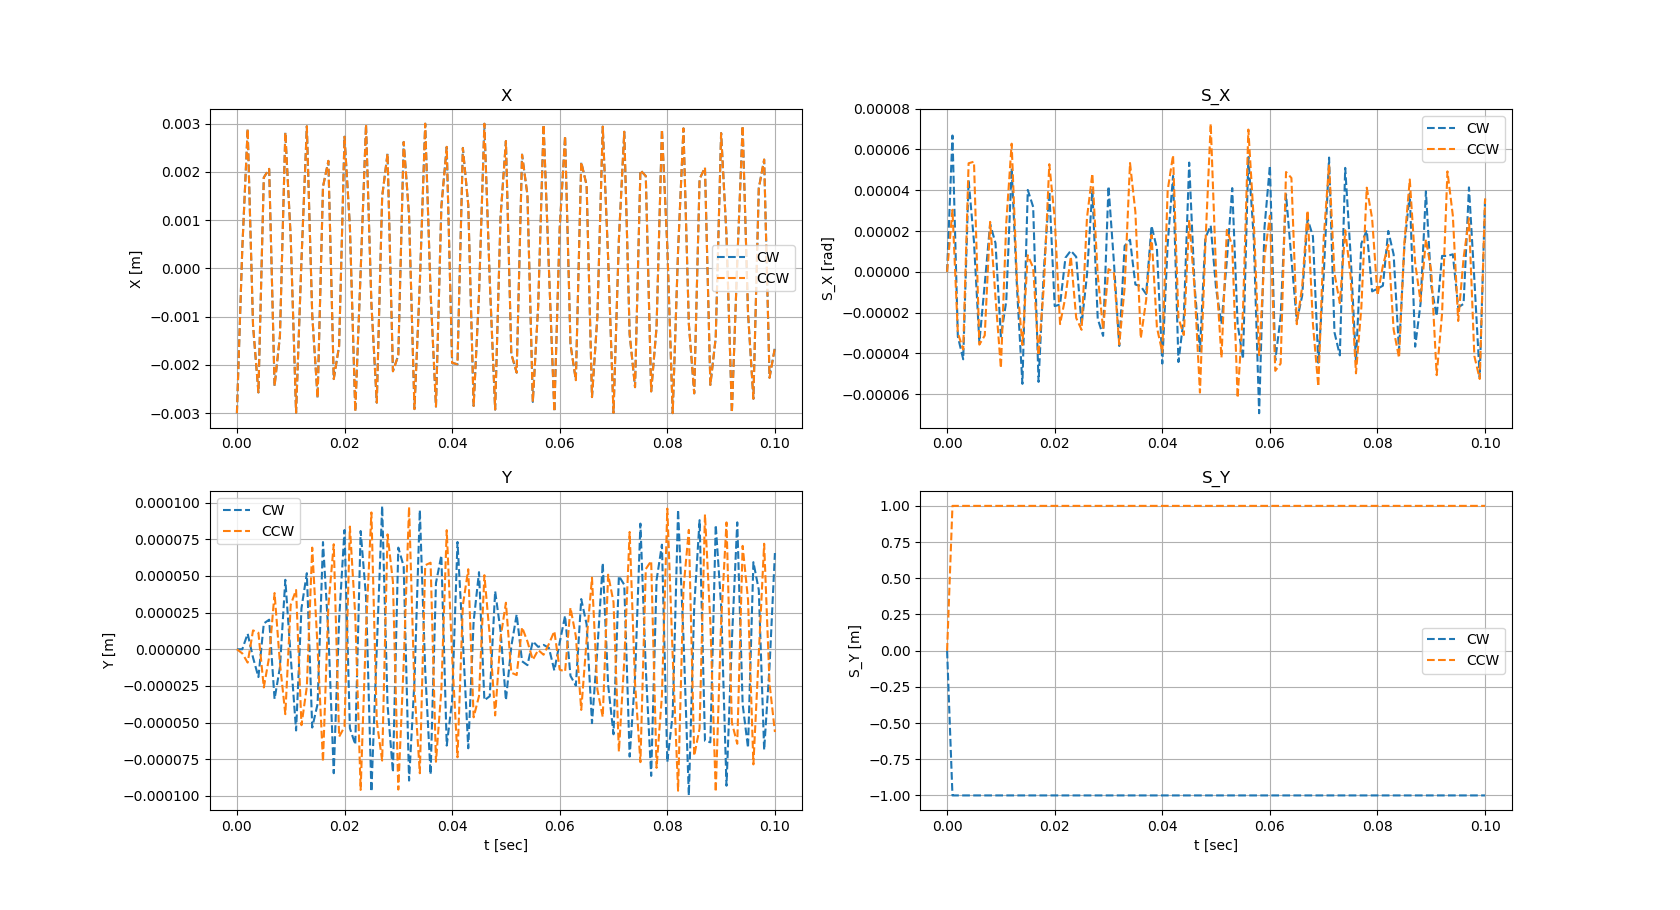
\includegraphics[scale=.3]{freeze/CALIB_MEAN_ZERO_SIGMA_ONE_PYGAUSS_another_run}
\end{frame}
\begin{frame}\frametitle{Spin freeze}
	\framesubtitle{$\theta\sim N(0,\sigma)$}
	 Another realization of the same distribution; this time there's no spin freeze.
	\centering
	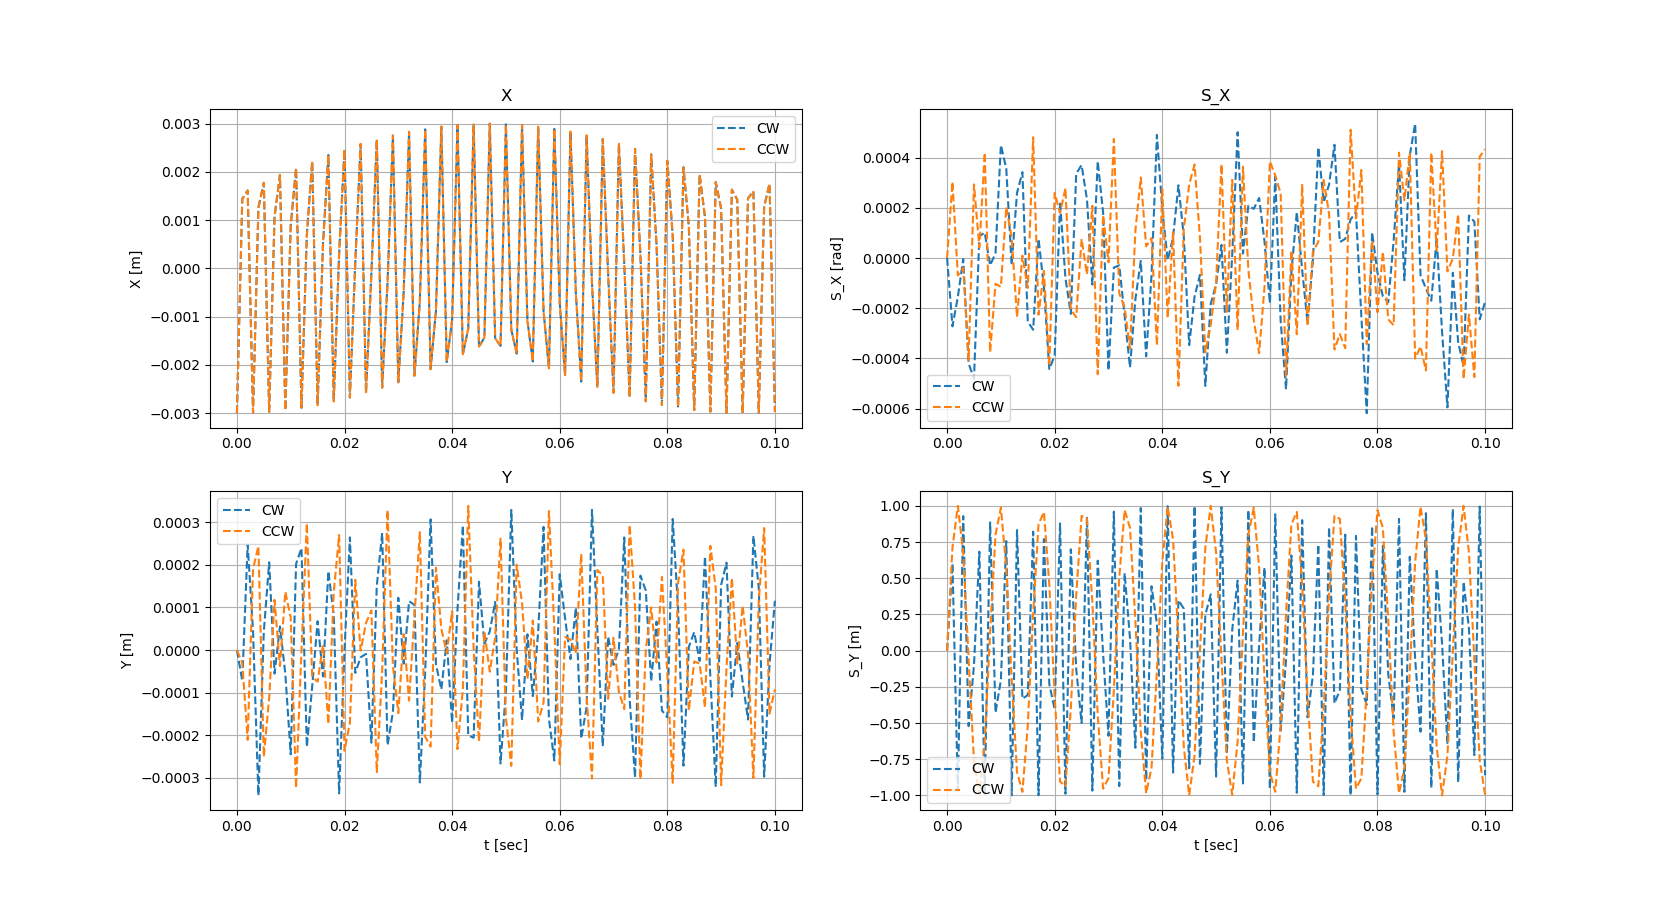
\includegraphics[scale=.3]{freeze/CALIB_MEAN_ZERO_SIGMA_ONE_PYGAUSS}
\end{frame}
\begin{frame}\frametitle{Look at the lattice as a whole}
	Hypothesis: something's wrong with the mean $B_x$ value.
	
	Simulation: Three values of $\sigma \in [1, 2, 3]\cdot 10^{-4}$ rad; 30 trials/value.
	\centering
	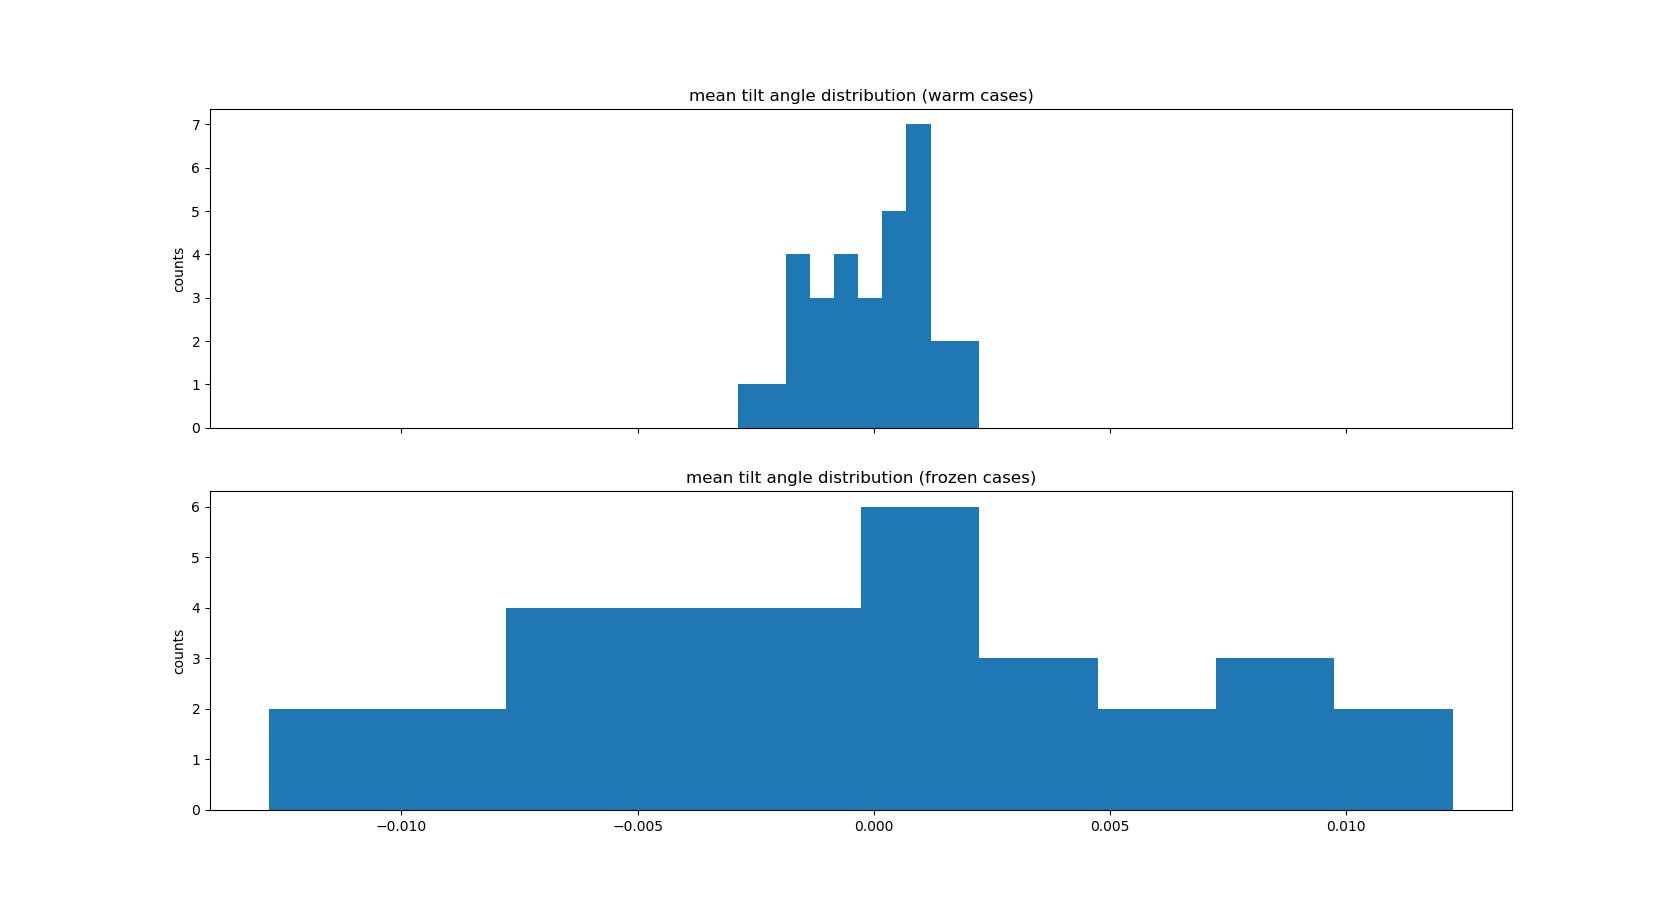
\includegraphics[scale=.3]{freeze/MEAN_TILT_ANGLE_WARM_FROZEN_HIST}
\end{frame}
\begin{frame}\frametitle{Look at particular WFs}
\framesubtitle{Tilted WF \#1 by $10^{-4}$ rad}
	Spin doesn't have a problem crossing the apex.
	\centering
	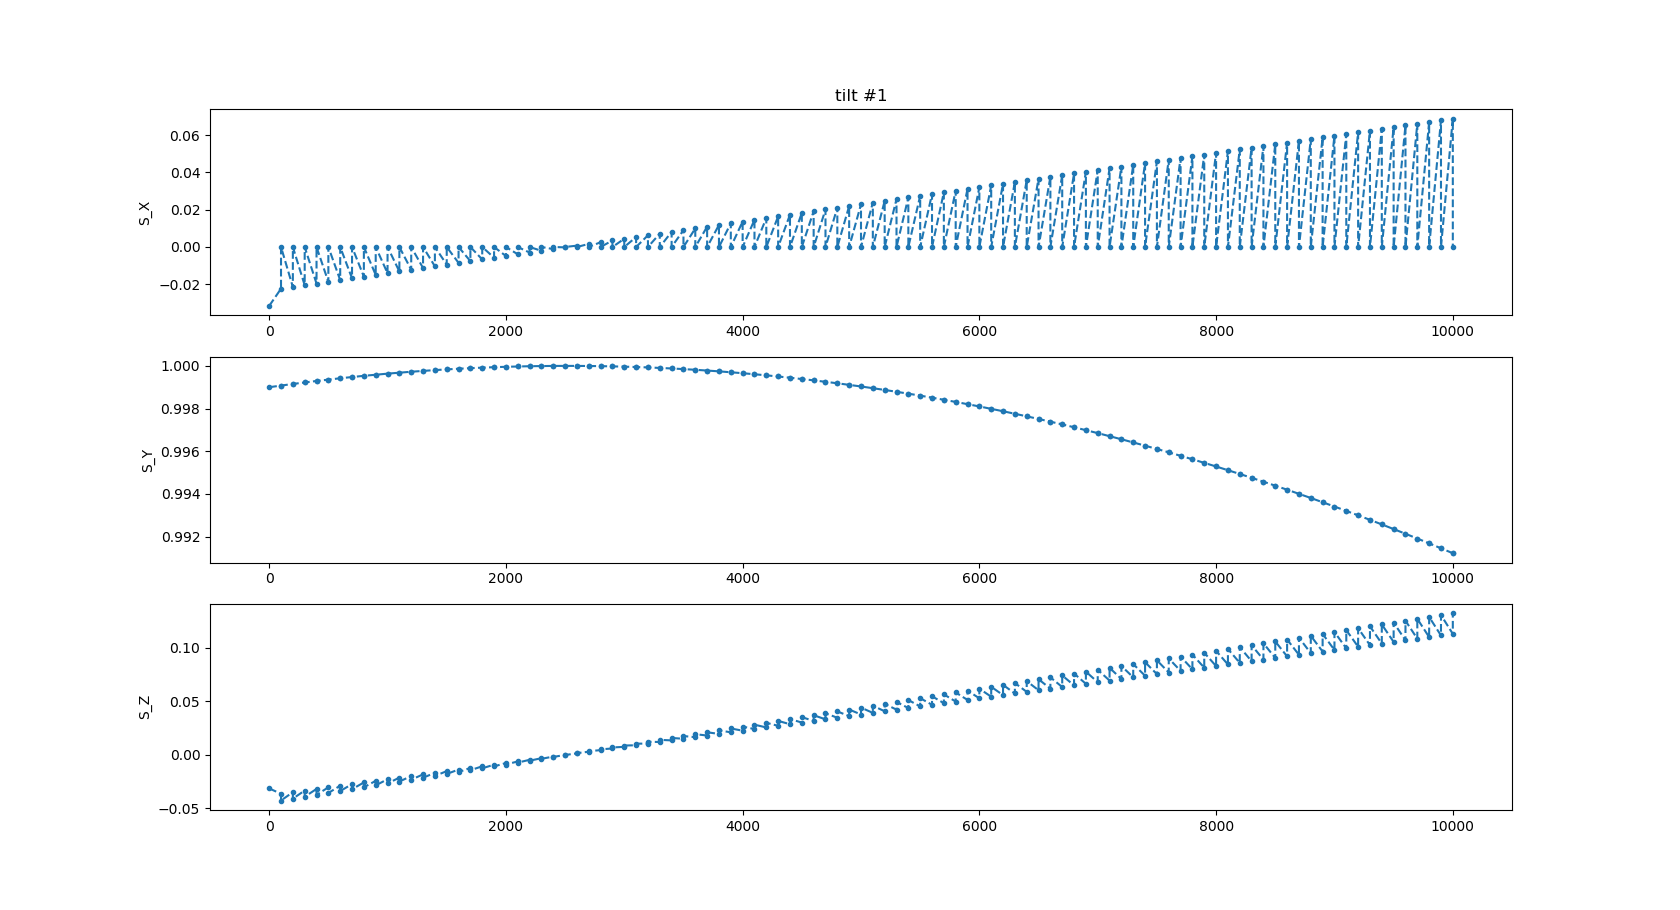
\includegraphics[scale=.3]{freeze/TITLS_TEST_1stWF_1e-4rad}
\end{frame}
\begin{frame}\frametitle{Look at particular WFs}
\framesubtitle{Tilted WF \#5 by $10^{-4}$ rad}
	Spin freeze at the top.
	\centering
	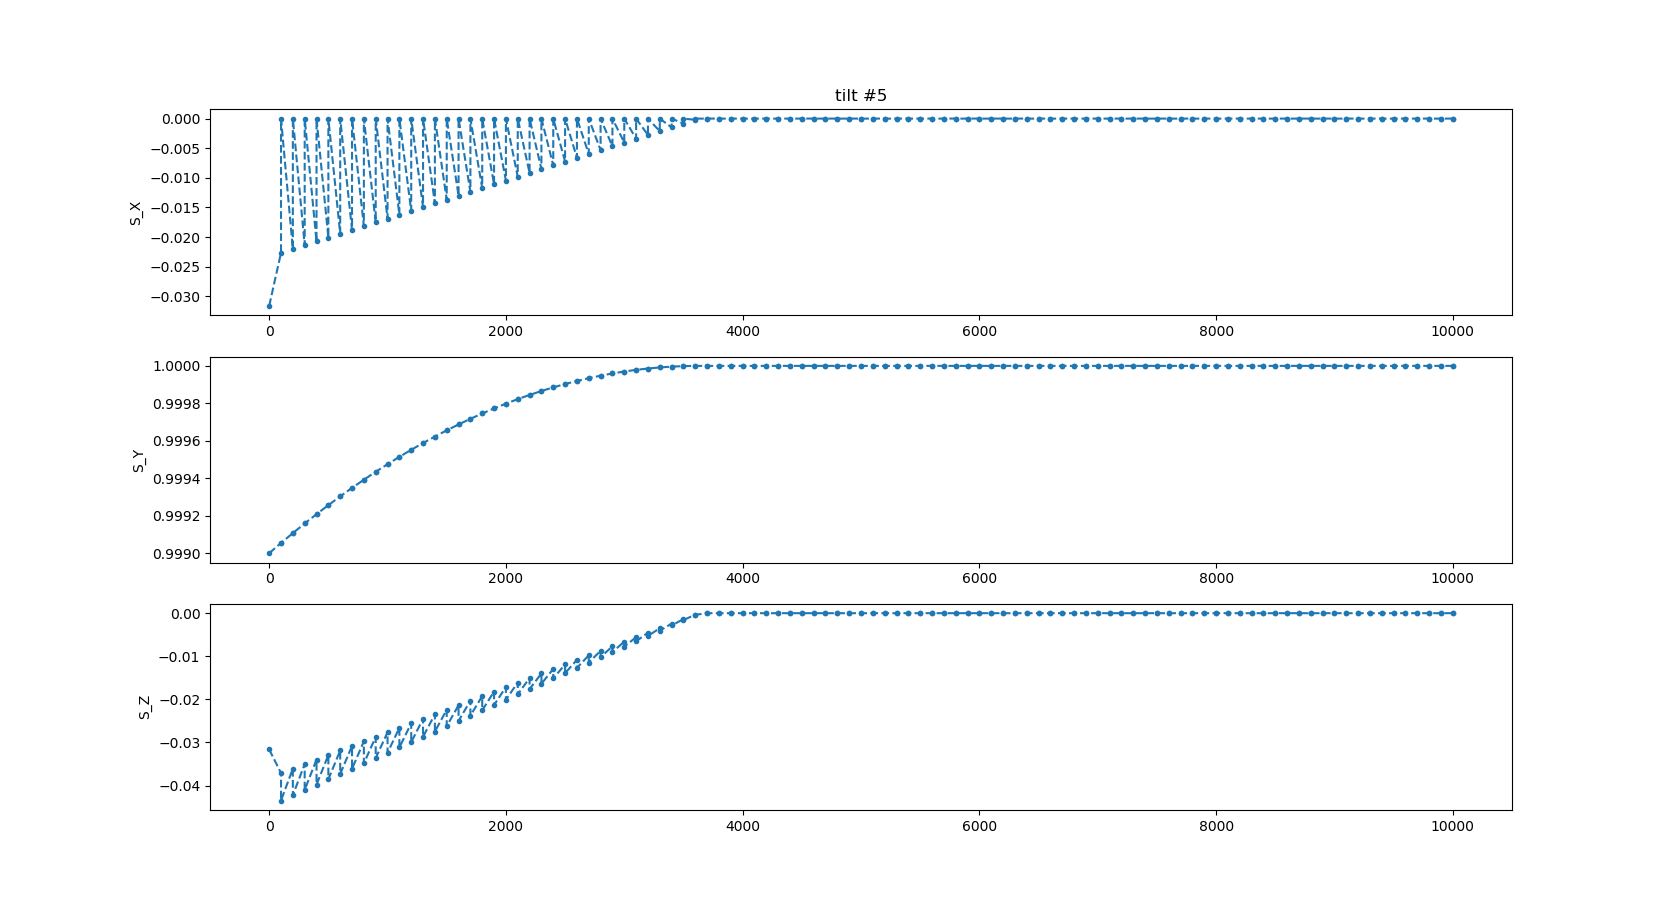
\includegraphics[scale=.3]{freeze/TITLS_TEST_5thWF_1e-4rad}
\end{frame}
\begin{frame}
	\frametitle{Probable causes}
	There's evidence that spin freeze is not caused by my crooked hands; Eremey also encountered that problem:
	\begin{itemize}
		\item Spin freeze is not a computational artifact; it's a resonance implicit in the mathematical model;
		\item it occurs whenever the spin vector gets into a certain, fairly wide altitude range close to $S_y = 1$.
	\end{itemize}
	And it looks like that range is dangerous in some places along the beamline, and not the others, seeing as tilting of WF \#\#1, 32, some others, doesn't cause freezing, whereas \#\#5, 8 does.
\end{frame}
\end{document}
